% ISBI 2027 4-page submission: entropy-gated triplet learning, focused on the like-for-like ablation the
% supervisor asked for. Plan / pre-registration: docs/plan/2026-10-08-entropy-ablation-isbi-submit-plan.md
% Template: official ISBI kit (spconf.sty, IEEEbib.bst; template_src/).
% Build:  latexmk -pdf paper.tex
% Numbers: every result number comes from generated/entropy_ablation_{macros,table}.tex, written by
%          analysis/entropy_ablation.py (only once all runs exist). Never type a result by hand.
% Placeholders: \TBD = a result not yet available (the paper is not finished while any remains);
%               \AUTHOR{...} = a statement only the authors can confirm (shown in blue).
\documentclass{article}
\usepackage{spconf,amsmath,amssymb,graphicx}
\usepackage{booktabs}
\usepackage{xcolor}
\usepackage{tikz}
\usetikzlibrary{positioning,arrows.meta,calc}
% compact bullet list (the template's enumitem is not installed here)
\newenvironment{tightlist}{\begin{list}{\textbullet}{\setlength{\itemsep}{0pt}\setlength{\parsep}{0pt}%
  \setlength{\topsep}{2pt}\setlength{\leftmargin}{12pt}\setlength{\labelwidth}{7pt}\setlength{\labelsep}{4pt}}}%
  {\end{list}}

\renewcommand{\topfraction}{0.95}\renewcommand{\textfraction}{0.05}\setcounter{topnumber}{3}
\newcommand{\TBD}[1][]{\textcolor{red}{\textbf{[TBD#1]}}}
\newcommand{\AUTHOR}[1]{\textcolor{blue}{#1}}
\IfFileExists{generated/entropy_ablation_macros.tex}{% generated by analysis/entropy_ablation.py on 2026-10-12 03:06 -- do not edit
\newcommand{\AblAslN}{6}
\newcommand{\AblAslMAP}{0.4381}
\newcommand{\AblAslMAPsd}{0.0042}
\newcommand{\AblAslMAUC}{0.9004}
\newcommand{\AblAslMAUCsd}{0.0017}
\newcommand{\AblAslMFone}{0.4504}
\newcommand{\AblAslMFonesd}{0.0049}
\newcommand{\AblAslMECE}{0.1281}
\newcommand{\AblAslMECEsd}{0.0005}
\newcommand{\AblAslHead}{0.7545}
\newcommand{\AblAslHeadsd}{0.0016}
\newcommand{\AblAslMedium}{0.4441}
\newcommand{\AblAslMediumsd}{0.0010}
\newcommand{\AblAslTail}{0.2854}
\newcommand{\AblAslTailsd}{0.0179}
\newcommand{\AblAslAnchors}{4.1}
\newcommand{\AblAslTriplets}{2.3}
\newcommand{\AblAslAnchorsFirst}{4.7}
\newcommand{\AblAslAnchorsLast}{3.4}
\newcommand{\AblAslYield}{56}
\newcommand{\AblNogateN}{6}
\newcommand{\AblNogateMAP}{0.4408}
\newcommand{\AblNogateMAPsd}{0.0012}
\newcommand{\AblNogateMAUC}{0.8996}
\newcommand{\AblNogateMAUCsd}{0.0035}
\newcommand{\AblNogateMFone}{0.4533}
\newcommand{\AblNogateMFonesd}{0.0049}
\newcommand{\AblNogateMECE}{0.1275}
\newcommand{\AblNogateMECEsd}{0.0066}
\newcommand{\AblNogateHead}{0.7534}
\newcommand{\AblNogateHeadsd}{0.0031}
\newcommand{\AblNogateMedium}{0.4430}
\newcommand{\AblNogateMediumsd}{0.0017}
\newcommand{\AblNogateTail}{0.3004}
\newcommand{\AblNogateTailsd}{0.0071}
\newcommand{\AblNogateAnchors}{8.0}
\newcommand{\AblNogateTriplets}{3.9}
\newcommand{\AblNogateAnchorsFirst}{8.0}
\newcommand{\AblNogateAnchorsLast}{8.0}
\newcommand{\AblNogateYield}{48}
\newcommand{\AblRandgateN}{6}
\newcommand{\AblRandgateMAP}{0.4395}
\newcommand{\AblRandgateMAPsd}{0.0044}
\newcommand{\AblRandgateMAUC}{0.9014}
\newcommand{\AblRandgateMAUCsd}{0.0009}
\newcommand{\AblRandgateMFone}{0.4509}
\newcommand{\AblRandgateMFonesd}{0.0076}
\newcommand{\AblRandgateMECE}{0.1314}
\newcommand{\AblRandgateMECEsd}{0.0035}
\newcommand{\AblRandgateHead}{0.7552}
\newcommand{\AblRandgateHeadsd}{0.0013}
\newcommand{\AblRandgateMedium}{0.4438}
\newcommand{\AblRandgateMediumsd}{0.0019}
\newcommand{\AblRandgateTail}{0.2919}
\newcommand{\AblRandgateTailsd}{0.0171}
\newcommand{\AblRandgateAnchors}{4.2}
\newcommand{\AblRandgateTriplets}{2.0}
\newcommand{\AblRandgateAnchorsFirst}{4.7}
\newcommand{\AblRandgateAnchorsLast}{3.5}
\newcommand{\AblRandgateYield}{49}
\newcommand{\AblGateN}{6}
\newcommand{\AblGateMAP}{0.4394}
\newcommand{\AblGateMAPsd}{0.0025}
\newcommand{\AblGateMAUC}{0.8999}
\newcommand{\AblGateMAUCsd}{0.0020}
\newcommand{\AblGateMFone}{0.4537}
\newcommand{\AblGateMFonesd}{0.0042}
\newcommand{\AblGateMECE}{0.1282}
\newcommand{\AblGateMECEsd}{0.0062}
\newcommand{\AblGateHead}{0.7544}
\newcommand{\AblGateHeadsd}{0.0026}
\newcommand{\AblGateMedium}{0.4439}
\newcommand{\AblGateMediumsd}{0.0013}
\newcommand{\AblGateTail}{0.2919}
\newcommand{\AblGateTailsd}{0.0103}
\newcommand{\AblRerunN}{2}
\newcommand{\AblRerunMAP}{0.4393}
\newcommand{\AblRerunMAPsd}{0.0010}
\newcommand{\AblRerunMAUC}{0.9023}
\newcommand{\AblRerunMAUCsd}{0.0008}
\newcommand{\AblRerunMFone}{0.4521}
\newcommand{\AblRerunMFonesd}{0.0002}
\newcommand{\AblRerunMECE}{0.1300}
\newcommand{\AblRerunMECEsd}{0.0008}
\newcommand{\AblRerunHead}{0.7548}
\newcommand{\AblRerunHeadsd}{0.0004}
\newcommand{\AblRerunMedium}{0.4434}
\newcommand{\AblRerunMediumsd}{0.0004}
\newcommand{\AblRerunTail}{0.2923}
\newcommand{\AblRerunTailsd}{0.0030}
\newcommand{\AblRerunAnchors}{4.2}
\newcommand{\AblRerunTriplets}{2.3}
\newcommand{\AblRerunAnchorsFirst}{4.7}
\newcommand{\AblRerunAnchorsLast}{3.4}
\newcommand{\AblRerunYield}{55}
\newcommand{\AblReproMAPEightySix}{0.0000}
\newcommand{\AblReproMAUCEightySix}{+0.0020}
\newcommand{\AblReproMFoneEightySix}{+0.0058}
\newcommand{\AblReproMECEEightySix}{-0.0025}
\newcommand{\AblReproHeadEightySix}{-0.0011}
\newcommand{\AblReproMediumEightySix}{-0.0016}
\newcommand{\AblReproTailEightySix}{+0.0051}
\newcommand{\AblReproMAPTenTwentyFour}{-0.0034}
\newcommand{\AblReproMAUCTenTwentyFour}{+0.0019}
\newcommand{\AblReproMFoneTenTwentyFour}{-0.0048}
\newcommand{\AblReproMECETenTwentyFour}{-0.0003}
\newcommand{\AblReproHeadTenTwentyFour}{-0.0012}
\newcommand{\AblReproMediumTenTwentyFour}{-0.0013}
\newcommand{\AblReproTailTenTwentyFour}{-0.0102}
\newcommand{\AblNFrontal}{11{,}973}
\newcommand{\AblNUnseen}{3{,}572}
\newcommand{\AblNIntervals}{35}
\newcommand{\AblNExcludeZero}{0}
\newcommand{\AblGateMinusNogateMAPmde}{0.0047}
\newcommand{\AblGateMinusNogateFront}{-0.0009}
\newcommand{\AblGateMinusNogateFrontlo}{-0.0049}
\newcommand{\AblGateMinusNogateFronthi}{+0.0031}
\newcommand{\AblGateMinusNogateFrontp}{0.594}
\newcommand{\AblGateMinusNogateFrontwins}{2/6}
\newcommand{\AblGateMinusNogateUnseen}{+0.0071}
\newcommand{\AblGateMinusNogateUnseenlo}{-0.0009}
\newcommand{\AblGateMinusNogateUnseenhi}{+0.0151}
\newcommand{\AblGateMinusNogateUnseenp}{0.062}
\newcommand{\AblGateMinusNogateUnseenwins}{5/6}
\newcommand{\AblGateMinusNogateMAP}{-0.0014}
\newcommand{\AblGateMinusNogateMAPlo}{-0.0048}
\newcommand{\AblGateMinusNogateMAPhi}{+0.0021}
\newcommand{\AblGateMinusNogateMAPp}{0.375}
\newcommand{\AblGateMinusNogateMAPwins}{2/6}
\newcommand{\AblGateMinusNogateMAPEns}{-0.0006}
\newcommand{\AblGateMinusNogateMAPEnslo}{-0.0046}
\newcommand{\AblGateMinusNogateMAPEnshi}{+0.0026}
\newcommand{\AblGateMinusNogateMAUC}{+0.0004}
\newcommand{\AblGateMinusNogateMAUClo}{-0.0041}
\newcommand{\AblGateMinusNogateMAUChi}{+0.0048}
\newcommand{\AblGateMinusNogateMAUCp}{0.656}
\newcommand{\AblGateMinusNogateMAUCwins}{4/6}
\newcommand{\AblGateMinusNogateMAUCEns}{+0.0002}
\newcommand{\AblGateMinusNogateMAUCEnslo}{-0.0009}
\newcommand{\AblGateMinusNogateMAUCEnshi}{+0.0011}
\newcommand{\AblGateMinusNogateMFone}{+0.0004}
\newcommand{\AblGateMinusNogateMFonelo}{-0.0033}
\newcommand{\AblGateMinusNogateMFonehi}{+0.0042}
\newcommand{\AblGateMinusNogateMFonep}{0.781}
\newcommand{\AblGateMinusNogateMFonewins}{4/6}
\newcommand{\AblGateMinusNogateMECE}{+0.0007}
\newcommand{\AblGateMinusNogateMECElo}{-0.0096}
\newcommand{\AblGateMinusNogateMECEhi}{+0.0111}
\newcommand{\AblGateMinusNogateMECEp}{0.594}
\newcommand{\AblGateMinusNogateMECEwins}{4/6}
\newcommand{\AblGateMinusNogateHead}{+0.0010}
\newcommand{\AblGateMinusNogateHeadlo}{-0.0038}
\newcommand{\AblGateMinusNogateHeadhi}{+0.0058}
\newcommand{\AblGateMinusNogateHeadp}{0.688}
\newcommand{\AblGateMinusNogateHeadwins}{3/6}
\newcommand{\AblGateMinusNogateHeadEns}{+0.0013}
\newcommand{\AblGateMinusNogateHeadEnslo}{+0.0003}
\newcommand{\AblGateMinusNogateHeadEnshi}{+0.0024}
\newcommand{\AblGateMinusNogateMedium}{+0.0008}
\newcommand{\AblGateMinusNogateMediumlo}{-0.0019}
\newcommand{\AblGateMinusNogateMediumhi}{+0.0035}
\newcommand{\AblGateMinusNogateMediump}{0.562}
\newcommand{\AblGateMinusNogateMediumwins}{4/6}
\newcommand{\AblGateMinusNogateMediumEns}{+0.0007}
\newcommand{\AblGateMinusNogateMediumEnslo}{-0.0003}
\newcommand{\AblGateMinusNogateMediumEnshi}{+0.0017}
\newcommand{\AblGateMinusNogateTail}{-0.0086}
\newcommand{\AblGateMinusNogateTaillo}{-0.0203}
\newcommand{\AblGateMinusNogateTailhi}{+0.0031}
\newcommand{\AblGateMinusNogateTailp}{0.125}
\newcommand{\AblGateMinusNogateTailwins}{1/6}
\newcommand{\AblGateMinusNogateTailEns}{-0.0053}
\newcommand{\AblGateMinusNogateTailEnslo}{-0.0222}
\newcommand{\AblGateMinusNogateTailEnshi}{+0.0077}
\newcommand{\AblGateMinusRandgateMAPmde}{0.0066}
\newcommand{\AblGateMinusRandgateFront}{-0.0008}
\newcommand{\AblGateMinusRandgateFrontlo}{-0.0085}
\newcommand{\AblGateMinusRandgateFronthi}{+0.0068}
\newcommand{\AblGateMinusRandgateFrontp}{0.938}
\newcommand{\AblGateMinusRandgateFrontwins}{4/6}
\newcommand{\AblGateMinusRandgateUnseen}{+0.0044}
\newcommand{\AblGateMinusRandgateUnseenlo}{-0.0023}
\newcommand{\AblGateMinusRandgateUnseenhi}{+0.0110}
\newcommand{\AblGateMinusRandgateUnseenp}{0.156}
\newcommand{\AblGateMinusRandgateUnseenwins}{4/6}
\newcommand{\AblGateMinusRandgateMAP}{0.0000}
\newcommand{\AblGateMinusRandgateMAPlo}{-0.0049}
\newcommand{\AblGateMinusRandgateMAPhi}{+0.0048}
\newcommand{\AblGateMinusRandgateMAPp}{0.969}
\newcommand{\AblGateMinusRandgateMAPwins}{2/6}
\newcommand{\AblGateMinusRandgateMAPEns}{+0.0018}
\newcommand{\AblGateMinusRandgateMAPEnslo}{-0.0032}
\newcommand{\AblGateMinusRandgateMAPEnshi}{+0.0061}
\newcommand{\AblGateMinusRandgateMAUC}{-0.0014}
\newcommand{\AblGateMinusRandgateMAUClo}{-0.0039}
\newcommand{\AblGateMinusRandgateMAUChi}{+0.0010}
\newcommand{\AblGateMinusRandgateMAUCp}{0.156}
\newcommand{\AblGateMinusRandgateMAUCwins}{1/6}
\newcommand{\AblGateMinusRandgateMAUCEns}{-0.0006}
\newcommand{\AblGateMinusRandgateMAUCEnslo}{-0.0014}
\newcommand{\AblGateMinusRandgateMAUCEnshi}{+0.0003}
\newcommand{\AblGateMinusRandgateMFone}{+0.0028}
\newcommand{\AblGateMinusRandgateMFonelo}{-0.0071}
\newcommand{\AblGateMinusRandgateMFonehi}{+0.0127}
\newcommand{\AblGateMinusRandgateMFonep}{0.594}
\newcommand{\AblGateMinusRandgateMFonewins}{3/6}
\newcommand{\AblGateMinusRandgateMECE}{-0.0032}
\newcommand{\AblGateMinusRandgateMECElo}{-0.0099}
\newcommand{\AblGateMinusRandgateMECEhi}{+0.0034}
\newcommand{\AblGateMinusRandgateMECEp}{0.406}
\newcommand{\AblGateMinusRandgateMECEwins}{2/6}
\newcommand{\AblGateMinusRandgateHead}{-0.0008}
\newcommand{\AblGateMinusRandgateHeadlo}{-0.0036}
\newcommand{\AblGateMinusRandgateHeadhi}{+0.0020}
\newcommand{\AblGateMinusRandgateHeadp}{0.562}
\newcommand{\AblGateMinusRandgateHeadwins}{3/6}
\newcommand{\AblGateMinusRandgateHeadEns}{0.0000}
\newcommand{\AblGateMinusRandgateHeadEnslo}{-0.0011}
\newcommand{\AblGateMinusRandgateHeadEnshi}{+0.0011}
\newcommand{\AblGateMinusRandgateMedium}{+0.0001}
\newcommand{\AblGateMinusRandgateMediumlo}{-0.0028}
\newcommand{\AblGateMinusRandgateMediumhi}{+0.0030}
\newcommand{\AblGateMinusRandgateMediump}{0.906}
\newcommand{\AblGateMinusRandgateMediumwins}{3/6}
\newcommand{\AblGateMinusRandgateMediumEns}{+0.0009}
\newcommand{\AblGateMinusRandgateMediumEnslo}{-0.0002}
\newcommand{\AblGateMinusRandgateMediumEnshi}{+0.0020}
\newcommand{\AblGateMinusRandgateTail}{0.0000}
\newcommand{\AblGateMinusRandgateTaillo}{-0.0160}
\newcommand{\AblGateMinusRandgateTailhi}{+0.0159}
\newcommand{\AblGateMinusRandgateTailp}{1.000}
\newcommand{\AblGateMinusRandgateTailwins}{4/6}
\newcommand{\AblGateMinusRandgateTailEns}{+0.0053}
\newcommand{\AblGateMinusRandgateTailEnslo}{-0.0161}
\newcommand{\AblGateMinusRandgateTailEnshi}{+0.0238}
\newcommand{\AblNogateMinusAslMAPmde}{0.0075}
\newcommand{\AblNogateMinusAslFront}{+0.0027}
\newcommand{\AblNogateMinusAslFrontlo}{-0.0032}
\newcommand{\AblNogateMinusAslFronthi}{+0.0087}
\newcommand{\AblNogateMinusAslFrontp}{0.281}
\newcommand{\AblNogateMinusAslFrontwins}{5/6}
\newcommand{\AblNogateMinusAslUnseen}{-0.0018}
\newcommand{\AblNogateMinusAslUnseenlo}{-0.0078}
\newcommand{\AblNogateMinusAslUnseenhi}{+0.0041}
\newcommand{\AblNogateMinusAslUnseenp}{0.438}
\newcommand{\AblNogateMinusAslUnseenwins}{2/6}
\newcommand{\AblNogateMinusAslMAP}{+0.0027}
\newcommand{\AblNogateMinusAslMAPlo}{-0.0028}
\newcommand{\AblNogateMinusAslMAPhi}{+0.0082}
\newcommand{\AblNogateMinusAslMAPp}{0.250}
\newcommand{\AblNogateMinusAslMAPwins}{5/6}
\newcommand{\AblNogateMinusAslMAPEns}{+0.0039}
\newcommand{\AblNogateMinusAslMAPEnslo}{+0.0008}
\newcommand{\AblNogateMinusAslMAPEnshi}{+0.0077}
\newcommand{\AblNogateMinusAslMAUC}{-0.0008}
\newcommand{\AblNogateMinusAslMAUClo}{-0.0036}
\newcommand{\AblNogateMinusAslMAUChi}{+0.0019}
\newcommand{\AblNogateMinusAslMAUCp}{0.562}
\newcommand{\AblNogateMinusAslMAUCwins}{2/6}
\newcommand{\AblNogateMinusAslMAUCEns}{-0.0001}
\newcommand{\AblNogateMinusAslMAUCEnslo}{-0.0014}
\newcommand{\AblNogateMinusAslMAUCEnshi}{+0.0010}
\newcommand{\AblNogateMinusAslMFone}{+0.0029}
\newcommand{\AblNogateMinusAslMFonelo}{-0.0021}
\newcommand{\AblNogateMinusAslMFonehi}{+0.0078}
\newcommand{\AblNogateMinusAslMFonep}{0.219}
\newcommand{\AblNogateMinusAslMFonewins}{5/6}
\newcommand{\AblNogateMinusAslMECE}{-0.0006}
\newcommand{\AblNogateMinusAslMECElo}{-0.0074}
\newcommand{\AblNogateMinusAslMECEhi}{+0.0063}
\newcommand{\AblNogateMinusAslMECEp}{1.000}
\newcommand{\AblNogateMinusAslMECEwins}{5/6}
\newcommand{\AblNogateMinusAslHead}{-0.0011}
\newcommand{\AblNogateMinusAslHeadlo}{-0.0035}
\newcommand{\AblNogateMinusAslHeadhi}{+0.0012}
\newcommand{\AblNogateMinusAslHeadp}{0.250}
\newcommand{\AblNogateMinusAslHeadwins}{2/6}
\newcommand{\AblNogateMinusAslHeadEns}{-0.0004}
\newcommand{\AblNogateMinusAslHeadEnslo}{-0.0014}
\newcommand{\AblNogateMinusAslHeadEnshi}{+0.0007}
\newcommand{\AblNogateMinusAslMedium}{-0.0010}
\newcommand{\AblNogateMinusAslMediumlo}{-0.0028}
\newcommand{\AblNogateMinusAslMediumhi}{+0.0007}
\newcommand{\AblNogateMinusAslMediump}{0.219}
\newcommand{\AblNogateMinusAslMediumwins}{2/6}
\newcommand{\AblNogateMinusAslMediumEns}{+0.0001}
\newcommand{\AblNogateMinusAslMediumEnslo}{-0.0009}
\newcommand{\AblNogateMinusAslMediumEnshi}{+0.0011}
\newcommand{\AblNogateMinusAslTail}{+0.0150}
\newcommand{\AblNogateMinusAslTaillo}{-0.0077}
\newcommand{\AblNogateMinusAslTailhi}{+0.0378}
\newcommand{\AblNogateMinusAslTailp}{0.188}
\newcommand{\AblNogateMinusAslTailwins}{5/6}
\newcommand{\AblNogateMinusAslTailEns}{+0.0165}
\newcommand{\AblNogateMinusAslTailEnslo}{+0.0041}
\newcommand{\AblNogateMinusAslTailEnshi}{+0.0327}
\newcommand{\AblGateMinusAslMAPmde}{0.0043}
\newcommand{\AblGateMinusAslFront}{+0.0018}
\newcommand{\AblGateMinusAslFrontlo}{-0.0044}
\newcommand{\AblGateMinusAslFronthi}{+0.0081}
\newcommand{\AblGateMinusAslFrontp}{0.500}
\newcommand{\AblGateMinusAslFrontwins}{4/6}
\newcommand{\AblGateMinusAslUnseen}{+0.0052}
\newcommand{\AblGateMinusAslUnseenlo}{-0.0036}
\newcommand{\AblGateMinusAslUnseenhi}{+0.0141}
\newcommand{\AblGateMinusAslUnseenp}{0.188}
\newcommand{\AblGateMinusAslUnseenwins}{4/6}
\newcommand{\AblGateMinusAslMAP}{+0.0013}
\newcommand{\AblGateMinusAslMAPlo}{-0.0018}
\newcommand{\AblGateMinusAslMAPhi}{+0.0045}
\newcommand{\AblGateMinusAslMAPp}{0.344}
\newcommand{\AblGateMinusAslMAPwins}{4/6}
\newcommand{\AblGateMinusAslMAPEns}{+0.0032}
\newcommand{\AblGateMinusAslMAPEnslo}{+0.0010}
\newcommand{\AblGateMinusAslMAPEnshi}{+0.0056}
\newcommand{\AblGateMinusAslMAUC}{-0.0005}
\newcommand{\AblGateMinusAslMAUClo}{-0.0029}
\newcommand{\AblGateMinusAslMAUChi}{+0.0019}
\newcommand{\AblGateMinusAslMAUCp}{0.625}
\newcommand{\AblGateMinusAslMAUCwins}{2/6}
\newcommand{\AblGateMinusAslMAUCEns}{+0.0001}
\newcommand{\AblGateMinusAslMAUCEnslo}{-0.0019}
\newcommand{\AblGateMinusAslMAUCEnshi}{+0.0015}
\newcommand{\AblGateMinusAslMFone}{+0.0033}
\newcommand{\AblGateMinusAslMFonelo}{-0.0007}
\newcommand{\AblGateMinusAslMFonehi}{+0.0074}
\newcommand{\AblGateMinusAslMFonep}{0.125}
\newcommand{\AblGateMinusAslMFonewins}{5/6}
\newcommand{\AblGateMinusAslMECE}{+0.0001}
\newcommand{\AblGateMinusAslMECElo}{-0.0065}
\newcommand{\AblGateMinusAslMECEhi}{+0.0067}
\newcommand{\AblGateMinusAslMECEp}{1.000}
\newcommand{\AblGateMinusAslMECEwins}{5/6}
\newcommand{\AblGateMinusAslHead}{-0.0001}
\newcommand{\AblGateMinusAslHeadlo}{-0.0032}
\newcommand{\AblGateMinusAslHeadhi}{+0.0029}
\newcommand{\AblGateMinusAslHeadp}{0.938}
\newcommand{\AblGateMinusAslHeadwins}{3/6}
\newcommand{\AblGateMinusAslHeadEns}{+0.0010}
\newcommand{\AblGateMinusAslHeadEnslo}{-0.0001}
\newcommand{\AblGateMinusAslHeadEnshi}{+0.0020}
\newcommand{\AblGateMinusAslMedium}{-0.0002}
\newcommand{\AblGateMinusAslMediumlo}{-0.0017}
\newcommand{\AblGateMinusAslMediumhi}{+0.0012}
\newcommand{\AblGateMinusAslMediump}{0.719}
\newcommand{\AblGateMinusAslMediumwins}{3/6}
\newcommand{\AblGateMinusAslMediumEns}{+0.0008}
\newcommand{\AblGateMinusAslMediumEnslo}{-0.0002}
\newcommand{\AblGateMinusAslMediumEnshi}{+0.0018}
\newcommand{\AblGateMinusAslTail}{+0.0065}
\newcommand{\AblGateMinusAslTaillo}{-0.0061}
\newcommand{\AblGateMinusAslTailhi}{+0.0191}
\newcommand{\AblGateMinusAslTailp}{0.219}
\newcommand{\AblGateMinusAslTailwins}{5/6}
\newcommand{\AblGateMinusAslTailEns}{+0.0112}
\newcommand{\AblGateMinusAslTailEnslo}{+0.0022}
\newcommand{\AblGateMinusAslTailEnshi}{+0.0206}
\newcommand{\AblRandgateMinusAslMAPmde}{0.0047}
\newcommand{\AblRandgateMinusAslFront}{+0.0027}
\newcommand{\AblRandgateMinusAslFrontlo}{-0.0014}
\newcommand{\AblRandgateMinusAslFronthi}{+0.0067}
\newcommand{\AblRandgateMinusAslFrontp}{0.188}
\newcommand{\AblRandgateMinusAslFrontwins}{4/6}
\newcommand{\AblRandgateMinusAslUnseen}{+0.0009}
\newcommand{\AblRandgateMinusAslUnseenlo}{-0.0104}
\newcommand{\AblRandgateMinusAslUnseenhi}{+0.0122}
\newcommand{\AblRandgateMinusAslUnseenp}{0.844}
\newcommand{\AblRandgateMinusAslUnseenwins}{4/6}
\newcommand{\AblRandgateMinusAslMAP}{+0.0014}
\newcommand{\AblRandgateMinusAslMAPlo}{-0.0021}
\newcommand{\AblRandgateMinusAslMAPhi}{+0.0048}
\newcommand{\AblRandgateMinusAslMAPp}{0.375}
\newcommand{\AblRandgateMinusAslMAPwins}{4/6}
\newcommand{\AblRandgateMinusAslMAPEns}{+0.0014}
\newcommand{\AblRandgateMinusAslMAPEnslo}{-0.0032}
\newcommand{\AblRandgateMinusAslMAPEnshi}{+0.0067}
\newcommand{\AblRandgateMinusAslMAUC}{+0.0010}
\newcommand{\AblRandgateMinusAslMAUClo}{-0.0002}
\newcommand{\AblRandgateMinusAslMAUChi}{+0.0021}
\newcommand{\AblRandgateMinusAslMAUCp}{0.094}
\newcommand{\AblRandgateMinusAslMAUCwins}{5/6}
\newcommand{\AblRandgateMinusAslMAUCEns}{+0.0007}
\newcommand{\AblRandgateMinusAslMAUCEnslo}{-0.0009}
\newcommand{\AblRandgateMinusAslMAUCEnshi}{+0.0019}
\newcommand{\AblRandgateMinusAslMFone}{+0.0005}
\newcommand{\AblRandgateMinusAslMFonelo}{-0.0101}
\newcommand{\AblRandgateMinusAslMFonehi}{+0.0112}
\newcommand{\AblRandgateMinusAslMFonep}{0.906}
\newcommand{\AblRandgateMinusAslMFonewins}{4/6}
\newcommand{\AblRandgateMinusAslMECE}{+0.0034}
\newcommand{\AblRandgateMinusAslMECElo}{-0.0006}
\newcommand{\AblRandgateMinusAslMECEhi}{+0.0073}
\newcommand{\AblRandgateMinusAslMECEp}{0.062}
\newcommand{\AblRandgateMinusAslMECEwins}{5/6}
\newcommand{\AblRandgateMinusAslHead}{+0.0007}
\newcommand{\AblRandgateMinusAslHeadlo}{-0.0008}
\newcommand{\AblRandgateMinusAslHeadhi}{+0.0022}
\newcommand{\AblRandgateMinusAslHeadp}{0.344}
\newcommand{\AblRandgateMinusAslHeadwins}{4/6}
\newcommand{\AblRandgateMinusAslHeadEns}{+0.0009}
\newcommand{\AblRandgateMinusAslHeadEnslo}{-0.0001}
\newcommand{\AblRandgateMinusAslHeadEnshi}{+0.0020}
\newcommand{\AblRandgateMinusAslMedium}{-0.0003}
\newcommand{\AblRandgateMinusAslMediumlo}{-0.0021}
\newcommand{\AblRandgateMinusAslMediumhi}{+0.0015}
\newcommand{\AblRandgateMinusAslMediump}{0.719}
\newcommand{\AblRandgateMinusAslMediumwins}{3/6}
\newcommand{\AblRandgateMinusAslMediumEns}{-0.0001}
\newcommand{\AblRandgateMinusAslMediumEnslo}{-0.0011}
\newcommand{\AblRandgateMinusAslMediumEnshi}{+0.0009}
\newcommand{\AblRandgateMinusAslTail}{+0.0065}
\newcommand{\AblRandgateMinusAslTaillo}{-0.0038}
\newcommand{\AblRandgateMinusAslTailhi}{+0.0168}
\newcommand{\AblRandgateMinusAslTailp}{0.125}
\newcommand{\AblRandgateMinusAslTailwins}{5/6}
\newcommand{\AblRandgateMinusAslTailEns}{+0.0059}
\newcommand{\AblRandgateMinusAslTailEnslo}{-0.0130}
\newcommand{\AblRandgateMinusAslTailEnshi}{+0.0276}
}{}
% Numbers copied (not computed) from existing, already-reported runs; sources:
%  - docs/paper/markov/paper.tex, Table "Patient-history Markov prior fed into the network" (v3 vs +prior vs withheld,
%    internal validation, flip TTA, SWA weights, seeds 42 and 1024, entropy-gated triplet model at 768 px)
%  - docs/result/2026-10-11-moe-matched-eval.md (MoE + prior, 2-seed means, with vs zero prior)
\newcommand{\MkBaseA}{0.4650}\newcommand{\MkPriorA}{0.4839}\newcommand{\MkWithA}{0.4624}
\newcommand{\MkBaseB}{0.4626}\newcommand{\MkPriorB}{0.4820}\newcommand{\MkWithB}{0.4663}
\newcommand{\MkEarlyBase}{0.4894}\newcommand{\MkEarlyPrior}{0.5276}\newcommand{\MkNEarlier}{5{,}759}
\newcommand{\MkMoeZero}{0.4663}\newcommand{\MkMoeWith}{0.4835}

\IfFileExists{generated/moe_baseline_macros.tex}{% generated by analysis/moe_table.py -- do not edit
\newcommand{\MoeTmMoeMAP}{-0.0008}
\newcommand{\MoeTmMoeMAPlo}{-0.0065}
\newcommand{\MoeTmMoeMAPhi}{+0.0043}
\newcommand{\MoeTmMoeMECE}{+0.0034}
\newcommand{\MoeTmMoeMECElo}{+0.0033}
\newcommand{\MoeTmMoeMECEhi}{+0.0035}
\newcommand{\MoeTmAslMAP}{+0.0035}
\newcommand{\MoeTmAslMAPlo}{-0.0018}
\newcommand{\MoeTmAslMAPhi}{+0.0101}
\newcommand{\MoeTmAslMECE}{+0.0024}
\newcommand{\MoeTmAslMECElo}{+0.0023}
\newcommand{\MoeTmAslMECEhi}{+0.0024}
\newcommand{\MoeMoeAslMAP}{+0.0043}
\newcommand{\MoeMoeAslMAPlo}{-0.0034}
\newcommand{\MoeMoeAslMAPhi}{+0.0123}
\newcommand{\MoeMoeAslMECE}{-0.0010}
\newcommand{\MoeMoeAslMECElo}{-0.0011}
\newcommand{\MoeMoeAslMECEhi}{-0.0009}
\newcommand{\MoeTmMoeFourMAP}{-0.0016}
\newcommand{\MoeTmMoeFourMAPlo}{-0.0051}
\newcommand{\MoeTmMoeFourMAPhi}{+0.0023}
\newcommand{\MoeTmMoeFourMECE}{+0.0030}
\newcommand{\MoeTmMoeFourMECElo}{+0.0029}
\newcommand{\MoeTmMoeFourMECEhi}{+0.0030}
}{}

\title{Entropy-Gated Triplet Cross-Memory-Bank Learning for Long-Tailed Multi-Label Chest X-Ray Classification}

% CONFIRM: author order and affiliations (taken from docs/paper/isbi/paper.tex); delete this line once confirmed
\name{\begin{tabular}[t]{c}Nguyen Trung Ky$^{\dagger}$ \quad Thien Nhan Pham$^{\star}$ \quad Huy Le Pham$^{\dagger}$ \\ Vladimir Fediunin$^{\star}$ \quad Grigorii Lukianov$^{\ddagger}$ \quad Christian Wagner$^{\star}$ \quad Shreyank Narayana Gowda$^{\star}$\end{tabular}}
\address{$^{\star}$ International University -- VNU, Ho Chi Minh City, Viet Nam\\
$^{\dagger}$ The University of Nottingham, Nottingham, United Kingdom\\
$^{\ddagger}$ University of Bath, Claverton Down, Bath, United Kingdom}

\begin{document}
\maketitle

\begin{abstract}
ConvNeXt with a query-based decoder is a simple, efficient chest X-ray classifier. Our previous CXR-LT 2026 entry improved it with a sparse mixture of experts (MoE) that adds parameters at inference and was reported with aggregate metrics only, so its effect on rare findings was not shown. We study training-time alternatives that leave the backbone unchanged: a triplet loss against a cross-batch memory bank with anchors chosen by predictive entropy, and a small patient-history Markov prior. Under one recipe, five seeds and seven metrics we compare the MoE, the entropy-gated triplet memory and the same with the Markov prior. \TBD[: results]
\end{abstract}

\begin{keywords}
Chest X-ray, long-tailed classification, triplet loss, cross-batch memory, predictive entropy
\end{keywords}



\section{Introduction}
\label{sec:intro}
Findings on chest radiographs are long-tailed and co-occur: in the CXR-LT 2026 Task~1 data~\cite{dong2026cxrlt}, built on PadChest~\cite{bustos2020padchest}, three of the 30 findings occur in over 10\% of our training images and seven in under 1\%. A ConvNeXt~\cite{liu2022convnext} with a query-based ML-Decoder head~\cite{ridnik2021mldecoder} trained with Asymmetric Loss (ASL)~\cite{ridnik2021asl} is a simple, efficient alternative to large transformers~\cite{dosovitskiy2021vit}.

Our previous entry~\cite{pham2026efficient} improved this model with a sparse MoE in the top stages and the decoder (third place, 0.4599 test mAP). Two problems remain: the experts and router add parameters at inference, and only aggregate metrics were reported, without a matched baseline or head, medium and tail results, so it is unknown whether the MoE helps rare findings or beats the plain model.

Here we ask whether the same ConvNeXt can instead be improved without extra inference-time parameters, by giving rare, co-occurring findings a stronger training signal and by using a patient's earlier studies. Therefore, in this paper we introduce new techniques to better fine-tune and improve ConvNeXt, a simple yet efficient model.

\newpage
\begin{figure}[t]
\centering
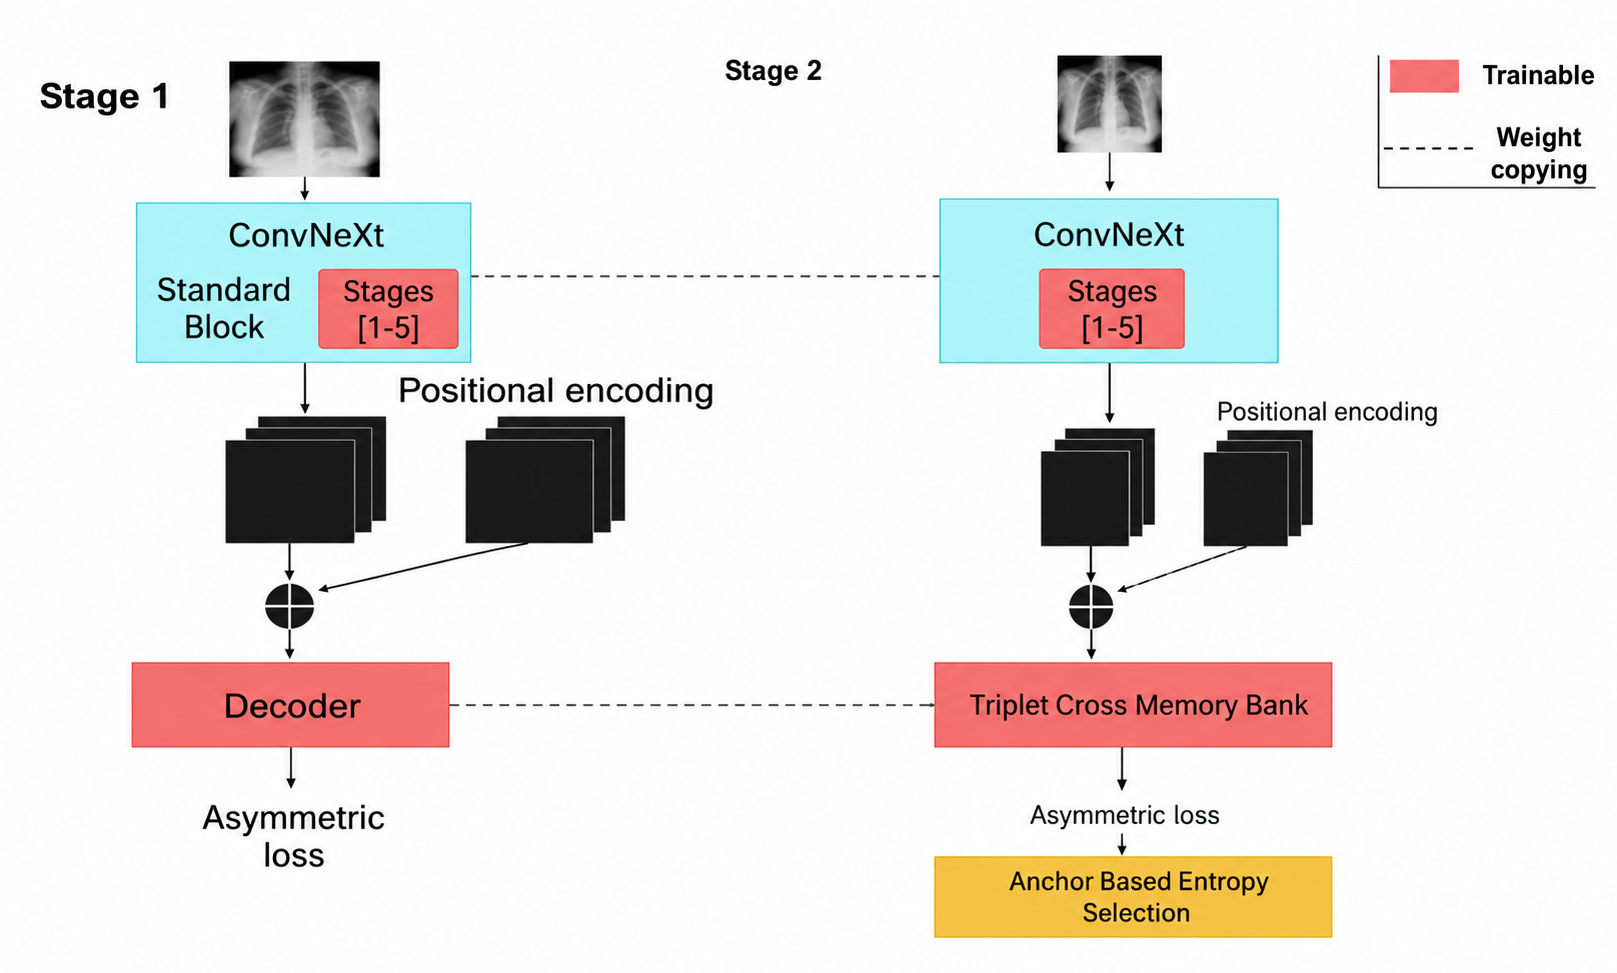
\includegraphics[width=0.97\linewidth]{figures/framework.png}
\caption{Two-stage training: Stage~1 with ASL only; Stage~2 adds the entropy-gated triplet loss with a cross-batch memory bank (Sec.~\ref{sec:method}).}
\label{fig:method}
\end{figure}

\begin{figure}[t]
\centering
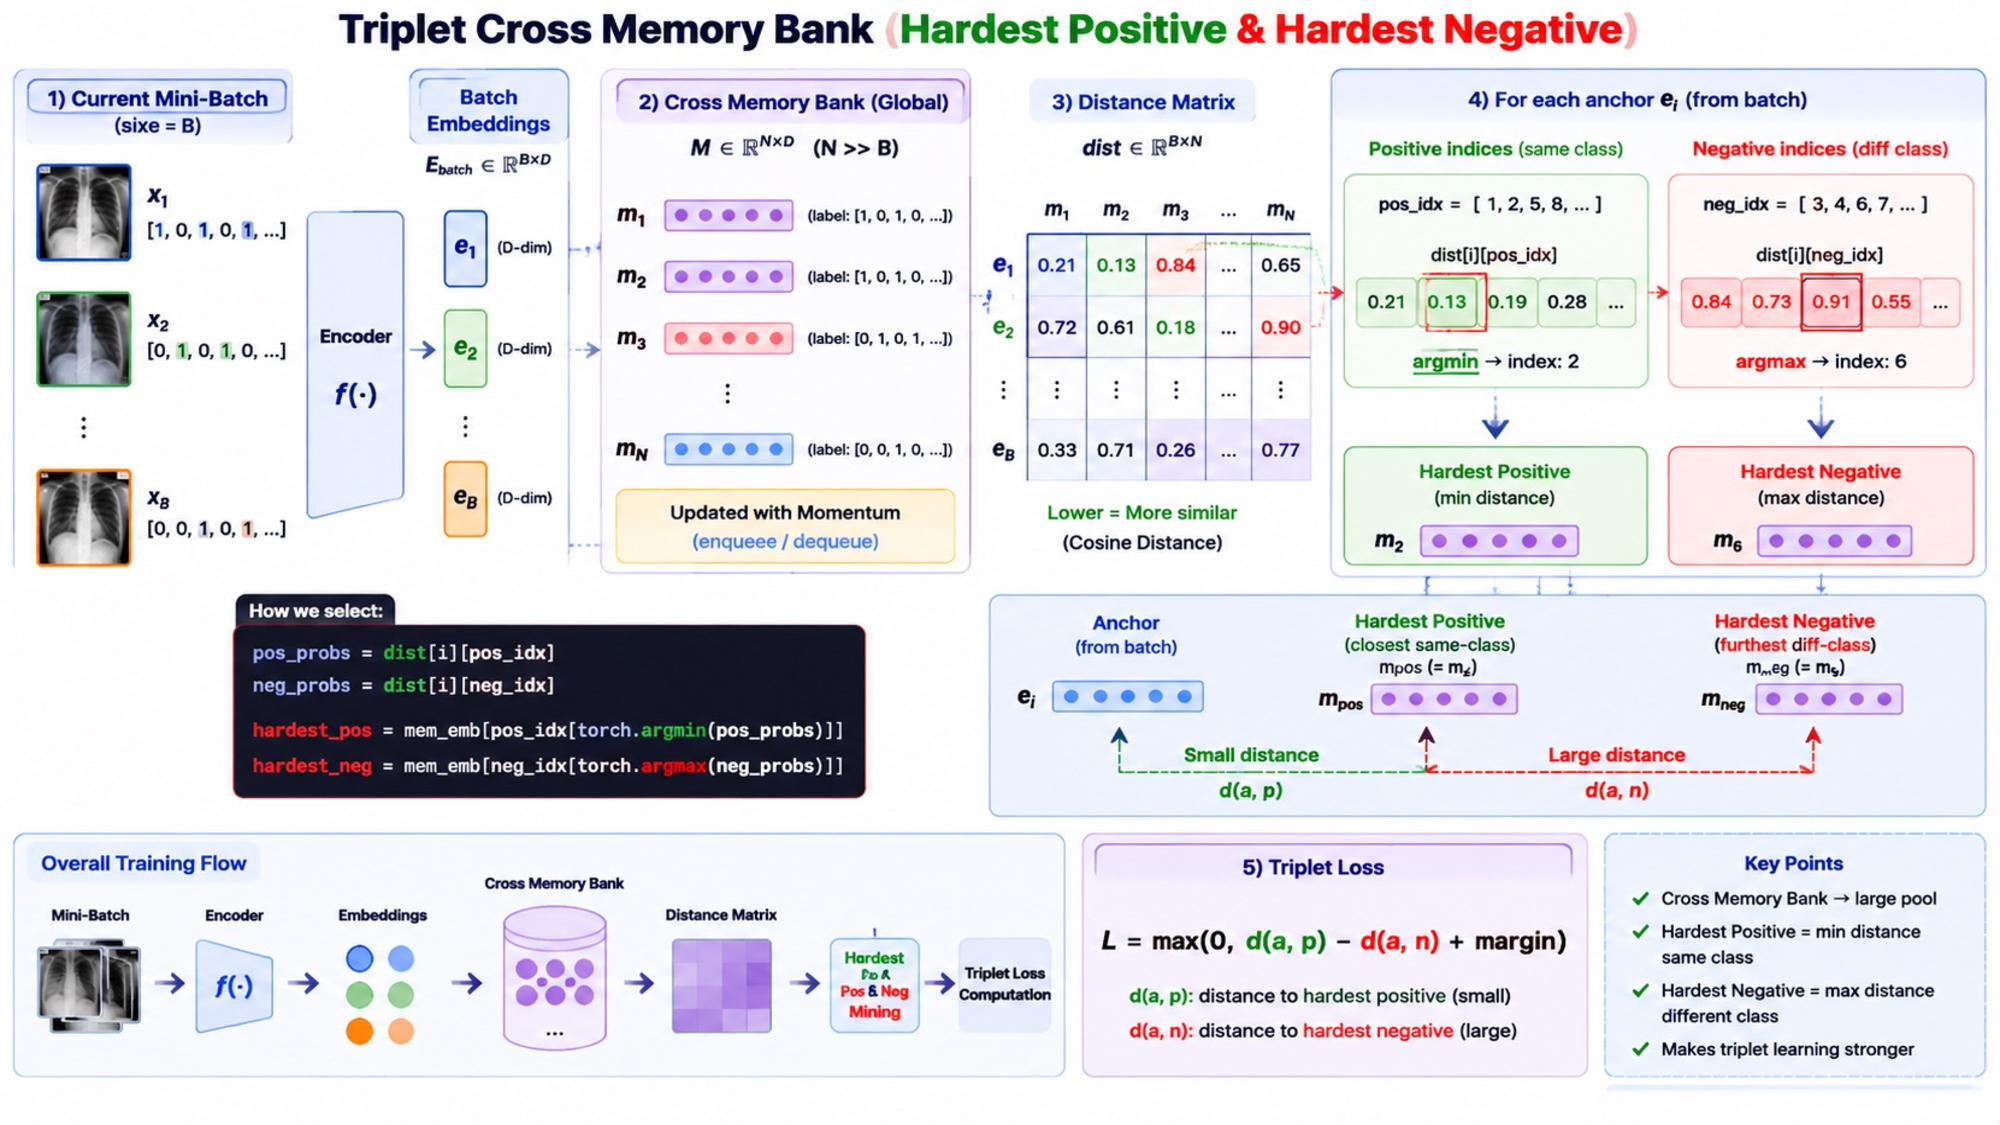
\includegraphics[width=0.97\linewidth]{figures/xbm.pdf}
\caption{Triplet cross-memory-bank pipeline (Eqs.~(\ref{eq:posneg})--(\ref{eq:triplet})). In the drawing, the ``hardest'' pairs are the easiest in the usual terminology (Sec.~\ref{sec:mining}), and the ``momentum'' update is the plain first-in-first-out queue of Sec.~\ref{sec:bank}.}
\label{fig:xbm}
\end{figure}

\section{Method}
\label{sec:method}



\subsection{Model}
The classifier is a ConvNeXt-B~\cite{liu2022convnext} with an added fifth stage of two blocks (total stride 64), followed by an ML-Decoder head~\cite{ridnik2021mldecoder}: the final feature map receives a 2D positional encoding~\cite{carion2020detr} and is projected to 768 channels, 30 fixed (non-trainable) label queries pass through two decoder layers, each with cross-attention to the feature map followed by self-attention among the queries, and a group-wise linear layer gives one logit $z_{ic}$ per finding (Fig.~\ref{fig:method}). Stage~1 trains this model end-to-end with ASL at $384$~px~\cite{pham2026efficient}; Stage~2 fine-tunes all of its trainable weights from that checkpoint. Only Stage~2 differs from our earlier entry. For metric learning we average the 30 decoded query embeddings of image $i$ and $\ell_2$-normalise the result, giving $e_i\in\mathbb{R}^{768}$.

\subsection{Cross-batch memory bank}
\label{sec:bank}
With batches of eight, few positive and negative pairs are available inside a batch, and the hardest pair found in a batch approximates the hardest pair in the data poorly. A first-in-first-out bank $\mathcal{M}$ holds the embeddings and multi-hot label vectors $\mathbf{y}$ of the 2{,}048 most recent training images (256 mini-batches of eight). After every step the batch's embeddings, detached from the graph, and labels replace the oldest entries, so each anchor sees a pool 256 times the size of a batch at no extra forward cost~\cite{wang2020xbm}. The entries come from slightly older encoder states.

\subsection{Entropy-gated anchors}
Rather than mining a triplet for every sample in the batch, we select anchors using the model's own predictive uncertainty, the criterion of active learning~\cite{settles2009active}. For each sample $x_i$ in a mini-batch $\mathcal{B}$ we compute the Shannon entropy of the softmax distribution over its $C=30$ classification logits, $p_\theta(y_c\mid x_i)=\exp z_{ic}/\sum_{k}\exp z_{ik}$,
\begin{equation}
H(x_i)=-\sum_{c=1}^{C}p_\theta(y_c\mid x_i)\,\log p_\theta(y_c\mid x_i),
\label{eq:entropy}
\end{equation}
and select as anchors the samples whose entropy is at or above the batch mean,
\begin{equation}
\mathcal{A}=\Bigl\{x_i\in\mathcal{B}:H(x_i)\ \ge\ \tfrac{1}{|\mathcal{B}|}\textstyle\sum_{x_j\in\mathcal{B}}H(x_j)\Bigr\}.
\label{eq:gate}
\end{equation}
On average \AblRerunAnchors{} of the eight images in a batch pass the gate (\AblRerunAnchorsFirst{} in the first epoch, \AblRerunAnchorsLast{} in the last epoch trained; two reruns of arm~C), and \AblRerunYield\% of these anchors find a valid positive and negative in the bank. The rationale is that an image classified with low entropy is already resolved and less informative to move in embedding space, so the triplet term should go to uncertain images; the ablation tests this, we do not assume it. Eq.~(\ref{eq:entropy}) treats the findings as one categorical distribution although they are separate binary labels; it is the rule we ablate, and a per-label (Bernoulli) entropy is a natural alternative.



\subsection{Mining and objective}
\label{sec:mining}
For an anchor $x_i\in\mathcal{A}$ with embedding $e_i$ and multi-hot label vector $\mathbf{y}_i$, positives are bank entries that share at least one finding with $x_i$ other than the five most frequent ones (Normal, pleural effusion, cardiomegaly, support devices, aortic elongation), and negatives share no finding (Fig.~\ref{fig:xbm}):
\begin{equation}
\begin{aligned}
\mathcal{P}(i)&=\{m\in\mathcal{M}:\mathbf{y}_m^{\top}D\,\mathbf{y}_i\ge 1\},\\
\mathcal{N}(i)&=\{m\in\mathcal{M}:\mathbf{y}_m^{\top}\mathbf{y}_i=0\},
\end{aligned}
\label{eq:posneg}
\end{equation}
where the diagonal matrix $D$ is zero at the five most frequent findings, so that two studies that are both Normal are not a positive pair. We take the closest positive and the farthest negative, $e_i^{+}=\arg\min_{m\in\mathcal{P}(i)}\lVert e_i-e_m\rVert_2$ and $e_i^{-}=\arg\max_{m\in\mathcal{N}(i)}\lVert e_i-e_m\rVert_2$. These are easy pairs rather than the hardest ones~\cite{hermans2017defense}; they are less exposed to noise in labels derived from reports, but we did not compare harder mining. Over the anchors $\mathcal{A}'\subseteq\mathcal{A}$ for which both sets are non-empty,
\begin{equation}
\mathcal{L}_{\mathrm{tri}}=\frac{1}{|\mathcal{A}'|}\sum_{x_i\in\mathcal{A}'}\max\bigl(0,\lVert e_i-e_i^{+}\rVert_2-\lVert e_i-e_i^{-}\rVert_2+\alpha\bigr),
\label{eq:triplet}
\end{equation}
and the objective is $\mathcal{L}=\mathcal{L}_{\mathrm{ASL}}+\lambda\,\mathcal{L}_{\mathrm{tri}}$ with $\alpha=0.5$ and $\lambda=0.1$. $\mathcal{L}_{\mathrm{ASL}}$ uses $\gamma_-=2$, $\gamma_+=0$, a probability margin of 0.05 and positive-term class weights proportional to $\log(1/f_c)$, with $f_c$ the training prevalence, normalised to mean one and clipped to $[0.5,2]$, so that rare findings contribute a larger positive gradient without destabilising the frequent ones. The bank, gate and triplet term exist only during training.

\subsection{Patient-history Markov prior}
\label{sec:markov}
Findings persist across a patient's studies. For each finding $c$, a two-state Markov chain estimated on the training fold gives its probability $\pi_c(y_{t-1})$ at a study from its presence at the patient's previous study. With $\bar\pi_c$ the training prevalence, the prior vector is $r_c=\operatorname{logit}\pi_c(y_{t-1})-\operatorname{logit}\bar\pi_c$, with a flag for an earlier study appended and $r=0$ when there is none. It offsets the label queries $Q_c$ before they attend to the image (Fig.~\ref{fig:markov}):
\begin{equation}
Q_c\leftarrow Q_c+r_c\,u_c+W r,\qquad c=1,\dots,30,
\label{eq:qprior}
\end{equation}
where $u_c$ and $W$ are zero-initialised, so training starts from the model without the prior. The objective, the entropy gate and the memory bank are unchanged: the offset acts before cross-attention, so it shifts the logits whose entropy selects the anchors and the decoded query embeddings that fill the bank. A post-prediction patient HMM that adds patient metadata uses the same chain (Fig.~\ref{fig:hmm}). Results are in Table~\ref{tab:ablation}.

\begin{figure}[t]
\centering
\resizebox{0.8\linewidth}{!}{%
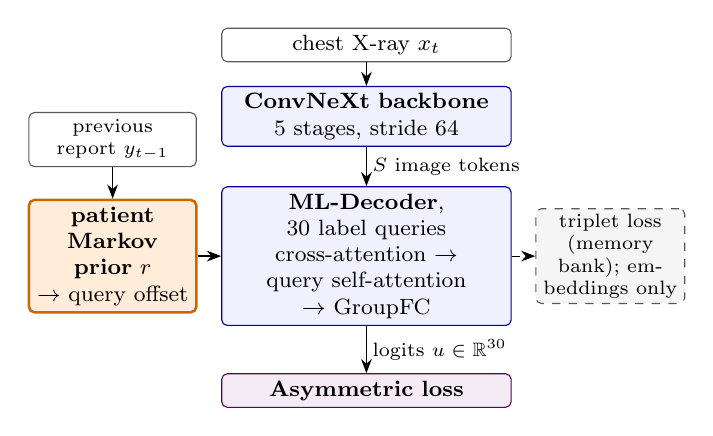
\begin{tikzpicture}[font=\footnotesize, node distance=3mm,
  box/.style={draw=blue!60!black, fill=blue!6, rounded corners=2pt, align=center, text width=3.5cm, inner sep=2.5pt},
  newbox/.style={draw=orange!80!black, fill=orange!15, rounded corners=2pt, align=center, text width=1.95cm, inner sep=2.5pt, line width=0.9pt},
  lossbox/.style={box, draw=violet!70!black, fill=violet!8},
  databox/.style={draw=gray!70!black, fill=white, rounded corners=2pt, align=center, inner sep=2.5pt},
  aux/.style={draw=gray!70!black, dashed, fill=gray!8, rounded corners=2pt, align=center, text width=1.75cm, inner sep=2pt, font=\scriptsize},
  arr/.style={-{Stealth[length=1.8mm]}},
  lab/.style={font=\scriptsize, right, inner sep=2pt}]
\node[databox, text width=3.5cm] (x) {chest X-ray $x_t$};
\node[box, below=of x] (bb) {\textbf{ConvNeXt backbone}\\5 stages, stride 64};
\node[box, below=5mm of bb] (dec) {\textbf{ML-Decoder}, 30 label queries\\cross-attention $\rightarrow$ query self-attention\\$\rightarrow$ GroupFC};
\node[lossbox, below=6mm of dec] (asl) {\textbf{Asymmetric loss}};
\node[aux, right=3mm of dec] (tri) {triplet loss (memory bank); embeddings only};
\node[newbox, left=3mm of dec] (pri) {\textbf{patient Markov prior} $r$\\$\rightarrow$ query offset};
\node[databox, text width=1.95cm, font=\scriptsize, above=4mm of pri] (rep) {previous report $y_{t-1}$};
\draw[arr] (x) -- (bb);
\draw[arr] (bb) -- node[lab]{$S$ image tokens} (dec);
\draw[arr] (dec) -- node[lab]{logits $u \in \mathbb{R}^{30}$} (asl);
\draw[arr, dashed] (dec) -- (tri);
\draw[arr] (rep) -- (pri);
\draw[arr, line width=0.9pt] (pri) -- (dec);
\end{tikzpicture}}
\caption{Where the Markov prior enters (orange): the patient-history prior $r$ offsets the ML-Decoder label queries.}
\label{fig:markov}
\end{figure}

\begin{figure}[t]
\centering
\resizebox{0.8\linewidth}{!}{%
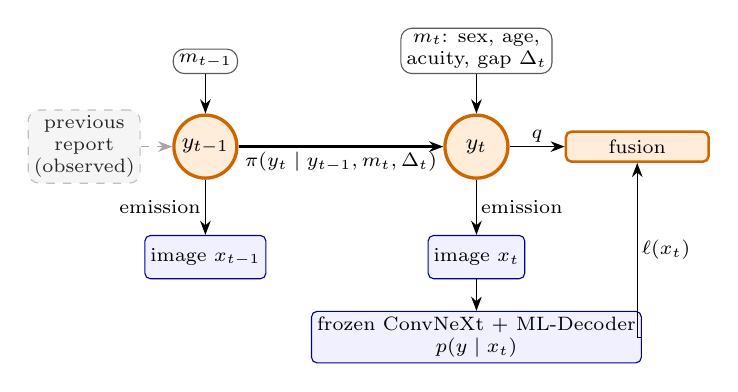
\begin{tikzpicture}[font=\footnotesize,
  st/.style={circle, draw=orange!80!black, fill=orange!15, line width=1.2pt, minimum size=8mm, inner sep=0pt},
  img/.style={draw=blue!60!black, fill=blue!6, rounded corners=2pt, align=center, inner sep=2pt, minimum height=5.5mm, font=\scriptsize},
  meta/.style={draw=gray!70!black, fill=white, rounded corners=4pt, align=center, inner sep=2pt, font=\scriptsize},
  aux/.style={draw=gray!50, dashed, fill=gray!8, rounded corners=4pt, align=center, inner sep=2pt, font=\scriptsize, text=gray!30!black},
  fuse/.style={draw=orange!80!black, fill=orange!15, rounded corners=2pt, align=center, inner sep=3pt, line width=0.9pt, font=\scriptsize},
  arr/.style={-{Stealth[length=1.8mm]}},
  lab/.style={font=\scriptsize, inner sep=1.5pt}]
\node[st] (y0) {$y_{t-1}$};
\node[st, right=26mm of y0] (y1) {$y_t$};
\node[meta, above=5mm of y0] (m0) {$m_{t-1}$};
\node[meta, above=5mm of y1] (m1) {$m_t$: sex, age,\\acuity, gap $\Delta_t$};
\node[aux, left=4mm of y0] (rep) {previous\\report\\(observed)};
\node[img, below=7mm of y0] (x0) {image $x_{t-1}$};
\node[img, below=7mm of y1] (x1) {image $x_t$};
\node[img, below=4mm of x1] (clf) {frozen ConvNeXt + ML-Decoder\\$p(y \mid x_t)$};
\node[fuse, right=7mm of y1, text width=1.6cm] (fz) {fusion};
\draw[arr, line width=1.2pt] (y0) -- node[lab, below]{$\pi(y_t \mid y_{t-1}, m_t, \Delta_t)$} (y1);
\draw[arr] (m0) -- (y0);
\draw[arr] (m1) -- (y1);
\draw[arr] (y0) -- node[lab, left]{emission} (x0);
\draw[arr] (y1) -- node[lab, right]{emission} (x1);
\draw[arr, dashed, draw=gray!70] (rep) -- (y0);
\draw[arr] (x1) -- (clf);
\draw[arr] (clf.east) -| node[lab, pos=0.75, right]{$\ell(x_t)$} (fz.south);
\draw[arr] (y1) -- node[lab, above]{$q$} (fz);
\end{tikzpicture}}
\caption{Post-prediction patient HMM: hidden finding states $y_t$, images and the frozen classifier as emissions, metadata and time gap $\Delta_t$ in the transition prior.}
\label{fig:hmm}
\end{figure}


\section{Results}
\label{sec:results}

\begin{table*}[t]
\caption{Unified test on the internal validation split (17{,}270 images): 768~px, seed 42, one run per system, so no s.d. All systems share the Stage-1 checkpoint and the schedule; scores use the SWA weights with horizontal-flip test-time augmentation. Head, medium, tail: mean AP over 3, 20, 7 findings. mECE: lower is better.}
\label{tab:ablation}
\centering
\small
\setlength{\tabcolsep}{4pt}
\resizebox{\textwidth}{!}{%
\begin{tabular}{lcccccccc}
\toprule
System & $n$ & mAP & mAUC & mF1 & mECE & head AP & medium AP & tail AP \\
\midrule
\IfFileExists{generated/seed42_768_table.tex}{% generated by analysis/seed42_768_table.py from unified_benchmark.json -- do not edit
% columns: system & n & mAP & mAUC & mF1 & mECE & head AP & medium AP & tail AP
ASL only (asymmetric loss) & 1 & 0.466 & 0.909 & 0.481 & 0.134 & 0.763 & 0.462 & 0.348 \\
Triplet Memory + Entropy & 1 & 0.461 & 0.912 & 0.467 & 0.135 & 0.764 & 0.462 & 0.326 \\
Triplet Memory + Entropy + Markov prior, history available & 1 & 0.484 & 0.916 & 0.493 & 0.134 & 0.772 & 0.480 & 0.372 \\
Triplet Memory + Entropy + Markov prior, history withheld & 1 & 0.462 & 0.912 & 0.474 & 0.137 & 0.764 & 0.459 & 0.342
 \\}{%
MoE (sparse mixture of experts) & & & & & & & & \\
Triplet Memory + Entropy & & & & & & & & \\
Triplet Memory + Entropy + Markov prior, history available & & & & & & & & \\
Triplet Memory + Entropy + Markov prior, history withheld & & & & & & & & \\}
\bottomrule
\end{tabular}}
\end{table*}

Our earlier entry, a sparse mixture of experts~\cite{pham2026efficient}, reported 0.405 mAP on this internal split at 384~px and 0.4599 on the official test set (third place); that recipe differs from ours, so these numbers are not comparable with Table~\ref{tab:ablation}. \TBD[: results text after the unified test: the three systems, paired differences over seeds with 95\% intervals and exact sign-flip tests, head, medium and tail AP, calibration]

\section{Discussion and Limitations}
\label{sec:discussion}
\TBD[: interpretation of the unified test] An earlier six-seed ablation at 512~px, run before this test, found no measurable effect of the entropy gate over using every image as an anchor. All results come from one internal validation fold that shares patients with the training set (77\% of its images) and includes lateral views (30\%), whereas the challenge test set is frontal and patient-disjoint; the absolute values are therefore likely optimistic. The Markov prior needs an earlier report of the same patient, which the test set does not provide, so only its withheld rows are test-like. The entropy in Eq.~(\ref{eq:entropy}) is a softmax over separate binary labels.

\section{Conclusion}
\label{sec:conclusion}
\TBD[: conclusion after the unified test]
\label{end-of-technical}% check_submission.py: everything above must end on page <= 4

\section{Compliance with Ethical Standards}
\label{sec:ethics}
\AUTHOR{This research study was conducted retrospectively using human subject data made available in open access by the CXR-LT 2026 challenge~\cite{dong2026cxrlt}, which is built on PadChest~\cite{bustos2020padchest}. Ethical approval was not required as confirmed by the license attached with the open access data.}

\section{Acknowledgments}
\label{sec:acknowledgments}
We thank the organisers of the CXR-LT 2026 challenge for the data. \AUTHOR{[Funding statement.] The authors have no relevant financial or non-financial interests to disclose.}

\bibliographystyle{IEEEbib}
{\footnotesize\setlength{\itemsep}{0pt}\setlength{\parskip}{0pt}\bibliography{refs}}

\end{document}
